% Modeling Assistant Learning Corpus

% This tex file was generated automatically by the createcorpus.py script.
% Generation time: 2022-08-11 03:12:36

\textbf{Legend:}
In the textual responses, items in \verb|${this format}| represent the parameters of
a parametrized response, which are computed and substituted at runtime from the general
template based on the specific mistake. Items [in square brackets] refer to optional
text which may or may not be included, depending on the student's knowledge.
Some of the resource responses, e.g., the ones used for the Player-Role pattern and
Abstraction-Occurrence pattern, are adapted from the textbook by
Lethbridge and Laganière~\cite{Lethbridge05}.

\section{Class mistakes}

\subsection{Class name mistakes}

\subsubsection{Plural class name}

Student element: Class. Instructor element: Class. \medskip

\noindent Level 1: Highlight solution  \medskip

\noindent Level 2: Text response: \medskip

\begin{tabular}{|p{0.9\linewidth}}
Remember that class names should be singular.
\end{tabular} \medskip

\noindent Level 3: Parametrized response: \medskip

\begin{tabular}{|p{0.9\linewidth}}
\verb|${stud_cls}| should be \verb|${inst_cls}|, using the singular.
\end{tabular} \medskip

\noindent Level 4: Resource response with Example: \medskip

\begin{tabular}{|p{0.9\linewidth}}
Please note these examples of correct vs incorrect class naming:
\end{tabular} \medskip

\begin{tabular}{ll}
\hline
\textcolor{red}{$\times$} Examples to avoid & \textcolor{ForestGreen}{\checkmark} Good class names \\
\hline
pilot & Pilot \\
Airplanes & Airplane  \\
AirlineData & Airline \\
\hline
\end{tabular} \medskip

\noindent Level 5: Resource response with Reference: \medskip

\begin{tabular}{|p{0.9\linewidth}}
Please review the \textit{Classes} part of the Class Diagram lecture.
\end{tabular} \medskip


\subsubsection{Software engineering term}

Student element: Class. Instructor element: Class. \medskip

\noindent Level 1: Highlight solution  \medskip

\noindent Level 2: Text response: \medskip

\begin{tabular}{|p{0.9\linewidth}}
Remember that a domain model should not contain software engineering terms.
\end{tabular} \medskip

\noindent Level 3: Parametrized response: \medskip

\begin{tabular}{|p{0.9\linewidth}}
\verb|${stud_cls}| contains a software engineering term (e.g., data, database, table, record), which does not belong in a domain model.
\end{tabular} \medskip

\noindent Level 4: Resource response with Example: \medskip

\begin{tabular}{|p{0.9\linewidth}}
Please note these examples of correct vs incorrect class naming:
\end{tabular} \medskip

\begin{tabular}{ll}
\hline
\textcolor{red}{$\times$} Examples to avoid & \textcolor{ForestGreen}{\checkmark} Good class names \\
\hline
pilot & Pilot \\
Airplanes & Airplane  \\
AirlineData & Airline \\
\hline
\end{tabular} \medskip

\noindent Level 5: Resource response with Reference: \medskip

\begin{tabular}{|p{0.9\linewidth}}
Please review the \textit{Classes} part of the Class Diagram lecture.
\end{tabular} \medskip


\subsection{Missing class}

Instructor element: Class. \medskip

\noindent Level 1: Highlight sentence(s) in problem statement referring to the instructor element \medskip

\noindent Level 2: Text response: \medskip

\begin{tabular}{|p{0.9\linewidth}}
Make sure you have modeled all the classes in the problem description.
\end{tabular} \medskip

\noindent Level 3: Highlight specific problem statement elements referring to the instructor element \medskip

\noindent Level 4: Parametrized response: \medskip

\begin{tabular}{|p{0.9\linewidth}}
Remember to add the \verb|${inst_cls}| class.
\end{tabular} \medskip

\noindent Level 5: Resource response with Reference: \medskip

\begin{tabular}{|p{0.9\linewidth}}
Please review the \textit{Classes} part of the Class Diagram lecture.
\end{tabular} \medskip



\section{Attribute mistakes}

\subsection{Attribute name mistakes}

\subsubsection{Bad attribute name spelling}

Student element: Attribute. Instructor element: Attribute. \medskip

\noindent Level 1: Highlight solution  \medskip

\noindent Level 2: Text response: \medskip

\begin{tabular}{|p{0.9\linewidth}}
Double check this attribute name.
\end{tabular} \medskip

\noindent Level 3: Parametrized response: \medskip

\begin{tabular}{|p{0.9\linewidth}}
The \verb|${stud_attr.cls}|.\verb|${stud_attr}| attribute is misspelled.[ Use the same spelling as the problem description.]
\end{tabular} \medskip

\noindent Level 4: Resource response with List multiple-choice quiz: \medskip

\begin{tabular}{|p{0.9\linewidth}}

Select all the correct attribute names from the list below.

\begin{itemize}
    \item[$\square$] needsReciept
    \item[$\boxtimes$] numberOfItems
    \item[$\square$] ID
    \item[$\square$] numItems
    \item[$\square$] Name
    \item[$\boxtimes$] identifier
\end{itemize}

\end{tabular} \medskip

\noindent Level 5: Resource response with Reference: \medskip

\begin{tabular}{|p{0.9\linewidth}}
Please review the \textit{Attribute} and \textit{Noun Analysis} parts of the Class Diagram lecture.
\end{tabular} \medskip


\subsection{Attribute in wrong class mistakes}

\subsubsection{Attribute misplaced}

Student element: Attribute. Instructor element: Attribute. \medskip

\noindent Level 1: Highlight solution  \medskip

\noindent Level 2: Text response: \medskip

\begin{tabular}{|p{0.9\linewidth}}
Can you think of a better place for this attribute?
\end{tabular} \medskip

\noindent Level 3: Parametrized response: \medskip

\begin{tabular}{|p{0.9\linewidth}}
The \verb|${stud_attr}| attribute does not belong in the \verb|${stud_attr.cls}| class. Where else can we place it?
\end{tabular} \medskip

\noindent Level 4: Parametrized response: \medskip

\begin{tabular}{|p{0.9\linewidth}}
The \verb|${stud_attr}| attribute belongs in the \verb|${inst_attr.cls}| class.
\end{tabular} \medskip

\noindent Level 5: Resource response with Reference: \medskip

\begin{tabular}{|p{0.9\linewidth}}
Please review the \textit{Attribute} and \textit{Noun Analysis} parts of the Class Diagram lecture.
\end{tabular} \medskip


\subsection{Extra attribute mistakes}

\subsubsection{Plural attribute}

Student element: Attribute. Instructor element: Attribute. \medskip

\noindent Level 1: Highlight solution  \medskip

\noindent Level 2: Text response: \medskip

\begin{tabular}{|p{0.9\linewidth}}
Double check this attribute name.
\end{tabular} \medskip

\noindent Level 3: Parametrized response: \medskip

\begin{tabular}{|p{0.9\linewidth}}
The \verb|${stud_attr.cls}|.\verb|${stud_attr}| attribute should be singular.
\end{tabular} \medskip

\noindent Level 4: Resource response with List multiple-choice quiz: \medskip

\begin{tabular}{|p{0.9\linewidth}}

Pick the classes which are modeled correctly with Umple.

\begin{itemize}
    \item[$\square$] class Student \{ courses; \}
    \item[$\square$] class Folder \{ List$<$File$>$ files; \}
    \item[$\boxtimes$] class Restaurant \{ 1 -- * Employee; \}
\end{itemize}

\end{tabular} \medskip

\noindent Level 5: Resource response with Reference: \medskip

\begin{tabular}{|p{0.9\linewidth}}
Please review the \textit{Attribute} and \textit{Noun Analysis} parts of the Class Diagram lecture.
\end{tabular} \medskip




\section{Relationship mistakes}

\subsection{Missing association/aggregation mistakes}

\subsubsection{Missing association}

Instructor element: Association. \medskip

\noindent Level 1: Highlight sentence(s) in problem statement referring to the instructor element \medskip

\noindent Level 2: Text response: \medskip

\begin{tabular}{|p{0.9\linewidth}}
How should this relationship be modeled?
\end{tabular} \medskip

\noindent Level 3: Parametrized response: \medskip

\begin{tabular}{|p{0.9\linewidth}}
How would you capture the relationship between \verb|${inst_assoc.end0.cls}| and \verb|${inst_assoc.end1.cls}|?
\end{tabular} \medskip

\noindent Level 4: Resource response with Reference: \medskip

\begin{tabular}{|p{0.9\linewidth}}
Please review the \textit{Composition vs. Aggregation vs. Association} section of 
the \textit{UML Class Diagram lecture slides} to 
better understand these relationships and where they are used.

\\
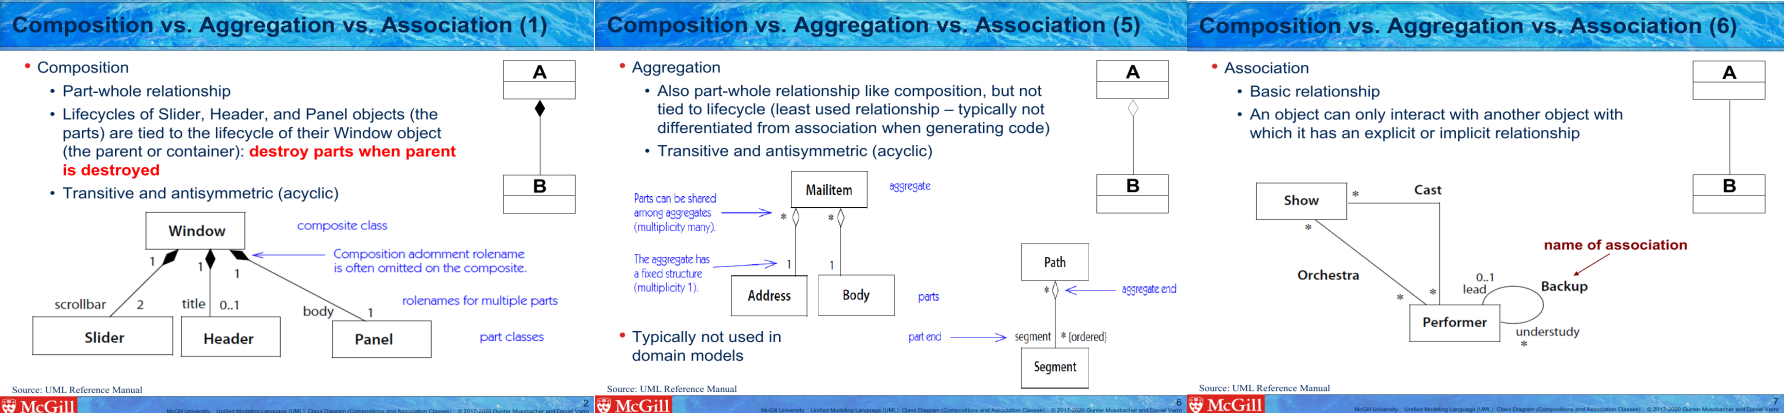
\includegraphics[width=0.9\textwidth]{images/composition_aggregation_association.png}
\end{tabular} \medskip


\subsubsection{Using attribute instead of association}

Student element: Attribute. Instructor element: Association end. \medskip

\noindent Level 1: Highlight solution  \medskip

\noindent Level 2: Text response: \medskip

\begin{tabular}{|p{0.9\linewidth}}
Remember that attributes are simple pieces of data.
\end{tabular} \medskip

\noindent Level 3: Parametrized response: \medskip

\begin{tabular}{|p{0.9\linewidth}}
\verb|${stud_attr}| should be its own class.
\end{tabular} \medskip

\noindent Level 4: Resource response with List multiple-choice quiz: \medskip

\begin{tabular}{|p{0.9\linewidth}}

Pick the class(es) modeled correctly in Umple.

\begin{itemize}
    \item[$\square$] class BankAccount \{ Client client; \}
    \item[$\boxtimes$] class BankAccount \{ * -- 1..2 Client clients; \}; class Client \{\}
    \item[$\square$] class BankAccount \{ 1..2 -- * Client clients; \}; class Client \{\}
    \item[$\square$] class Loan \{ libraryPatron; \}
\end{itemize}

\end{tabular} \medskip

\noindent Level 5: Resource response with Reference: \medskip

\begin{tabular}{|p{0.9\linewidth}}
Please review the \textit{Composition vs. Aggregation vs. Association} section of 
the \textit{UML Class Diagram lecture slides} to 
better understand these relationships and where they are used.

\\
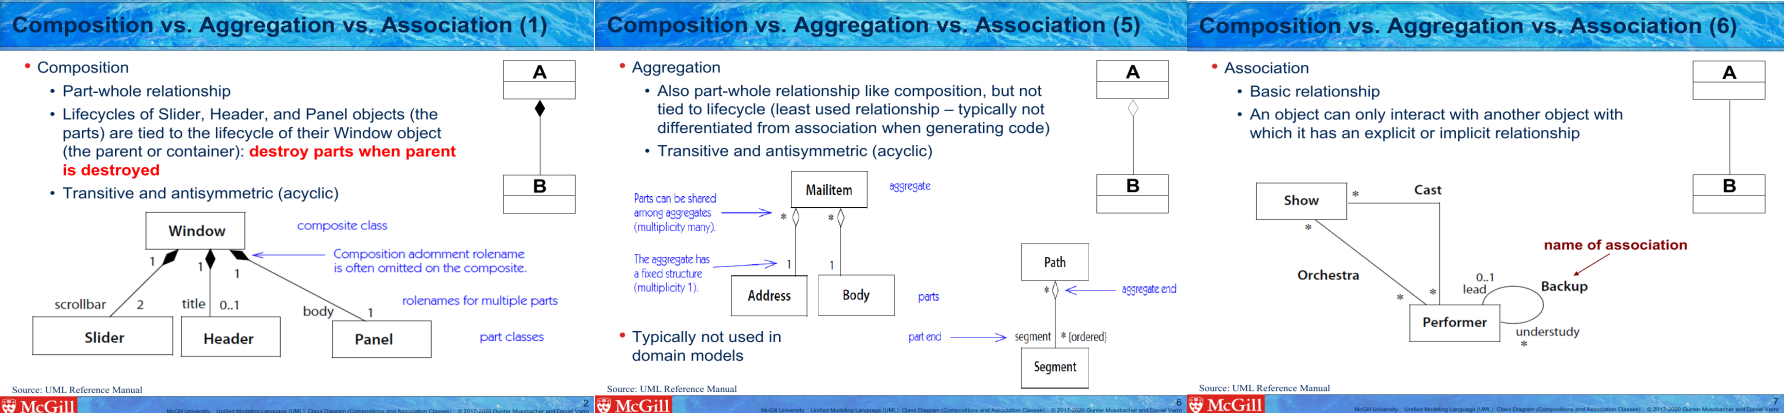
\includegraphics[width=0.9\textwidth]{images/composition_aggregation_association.png}
\end{tabular} \medskip


\subsection{Multiplicity mistakes}

\subsubsection{Wrong multiplicity}

Student element: Association end. Instructor element: Association end. \medskip

\noindent Level 1: Highlight solution  \medskip

\noindent Level 2: Text response: \medskip

\begin{tabular}{|p{0.9\linewidth}}
Double check this association.
\end{tabular} \medskip

\noindent Level 3: Text response: \medskip

\begin{tabular}{|p{0.9\linewidth}}
The multiplicity for this association end is incorrect.
\end{tabular} \medskip

\noindent Level 4: Parametrized response: \medskip

\begin{tabular}{|p{0.9\linewidth}}
How many \verb|${stud_assocend.opposite.cls}| instances does a \verb|${stud_assocend.cls}| have?
\end{tabular} \medskip

\noindent Level 5: Resource response with List multiple-choice quiz: \medskip

\begin{tabular}{|p{0.9\linewidth}}

Pick the association(s) with correct multiplicities:

\begin{itemize}
    \item[$\square$] 1 EmployeeRole -- 1 Person;
    \item[$\boxtimes$] * Episode -- 1 TvSeries;
    \item[$\square$] * Bank -- 1 Client;
    \item[$\square$] * Client -- 1 BankAccount;
    \item[$\boxtimes$] 0..2 Loan -- 1 Client;
    \item[$\square$] * Person -- 1 EmployeeRole;
    \item[$\boxtimes$] * EmployeeRole -- 1 Person;
\end{itemize}

\end{tabular} \medskip

\noindent Level 6: Resource response with Reference: \medskip

\begin{tabular}{|p{0.9\linewidth}}
Please review the \textit{multiplicities} part of the Class Diagram lecture.
\end{tabular} \medskip


\subsection{Role name mistakes}

\subsubsection{Missing role name}

Student element: Association end. Instructor element: Association end. \medskip

\noindent Level 1: Highlight solution  \medskip

\noindent Level 2: Text response: \medskip

\begin{tabular}{|p{0.9\linewidth}}
Can you model this relationship more precisely?
\end{tabular} \medskip

\noindent Level 3: Parametrized response: \medskip

\begin{tabular}{|p{0.9\linewidth}}
The relationship between \verb|${stud_assocend.cls}| and \verb|${stud_assocend.opposite.cls}| is missing a role name.
\end{tabular} \medskip

\noindent Level 4: Resource response with Reference: \medskip

\begin{tabular}{|p{0.9\linewidth}}
Can you think of appropriate \textit{role names}
for this relationship? Role names help identify the role a class plays in a
relationship and are particularly important if there is more than one relationship
between the same two classes.

\\
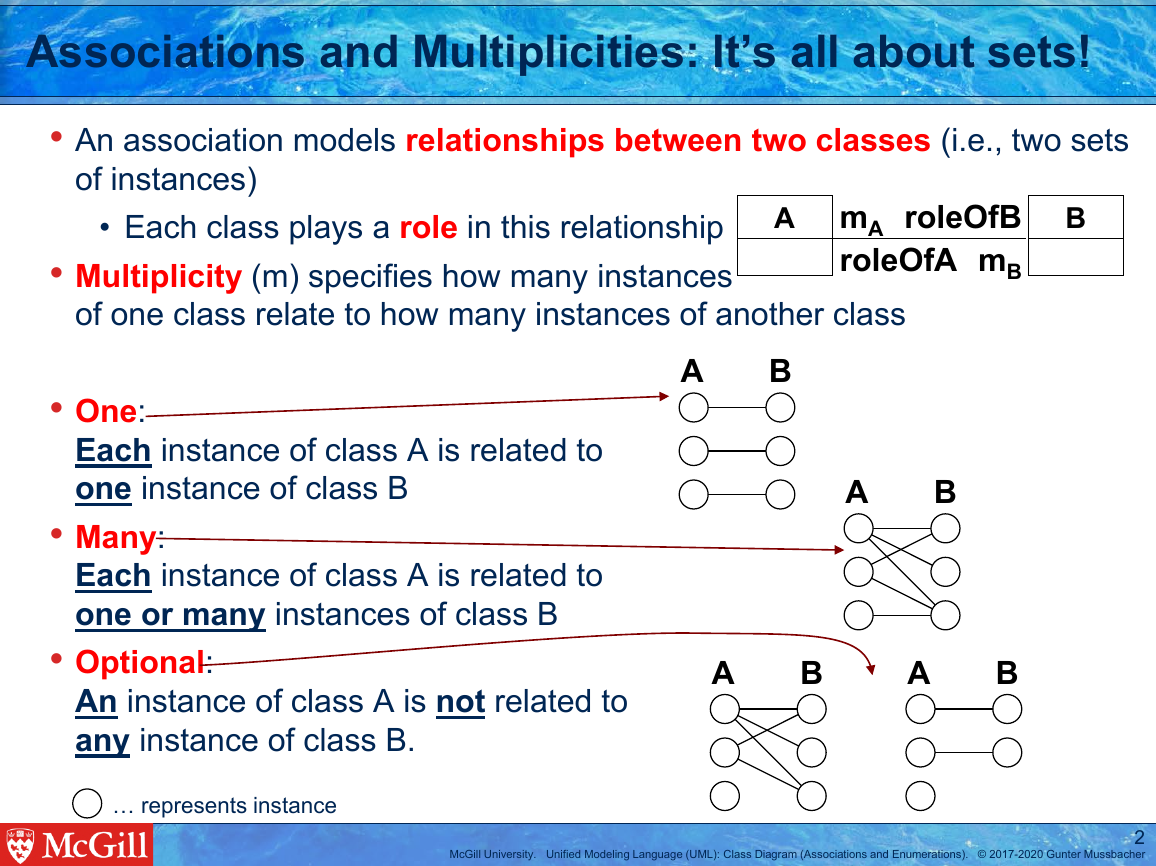
\includegraphics[width=0.6\textwidth]{images/role_name.png}
\end{tabular} \medskip


\subsubsection{Wrong role name but correct association}

Student element: Attribute.  \medskip

\noindent Level 1: Highlight solution  \medskip

\noindent Level 2: Text response: \medskip

\begin{tabular}{|p{0.9\linewidth}}
Double check this role name.
\end{tabular} \medskip

\noindent Level 3: Parametrized response: \medskip

\begin{tabular}{|p{0.9\linewidth}}
The \verb|${stud_assocend}| role name is not correct.
\end{tabular} \medskip

\noindent Level 4: Parametrized response: \medskip

\begin{tabular}{|p{0.9\linewidth}}
The \verb|${stud_assocend}| role name should be changed to \verb|${inst_assocend}|.
\end{tabular} \medskip

\noindent Level 5: Resource response with Reference: \medskip

\begin{tabular}{|p{0.9\linewidth}}
Can you think of appropriate \textit{role names}
for this relationship? Role names help identify the role a class plays in a
relationship and are particularly important if there is more than one relationship
between the same two classes.

\\
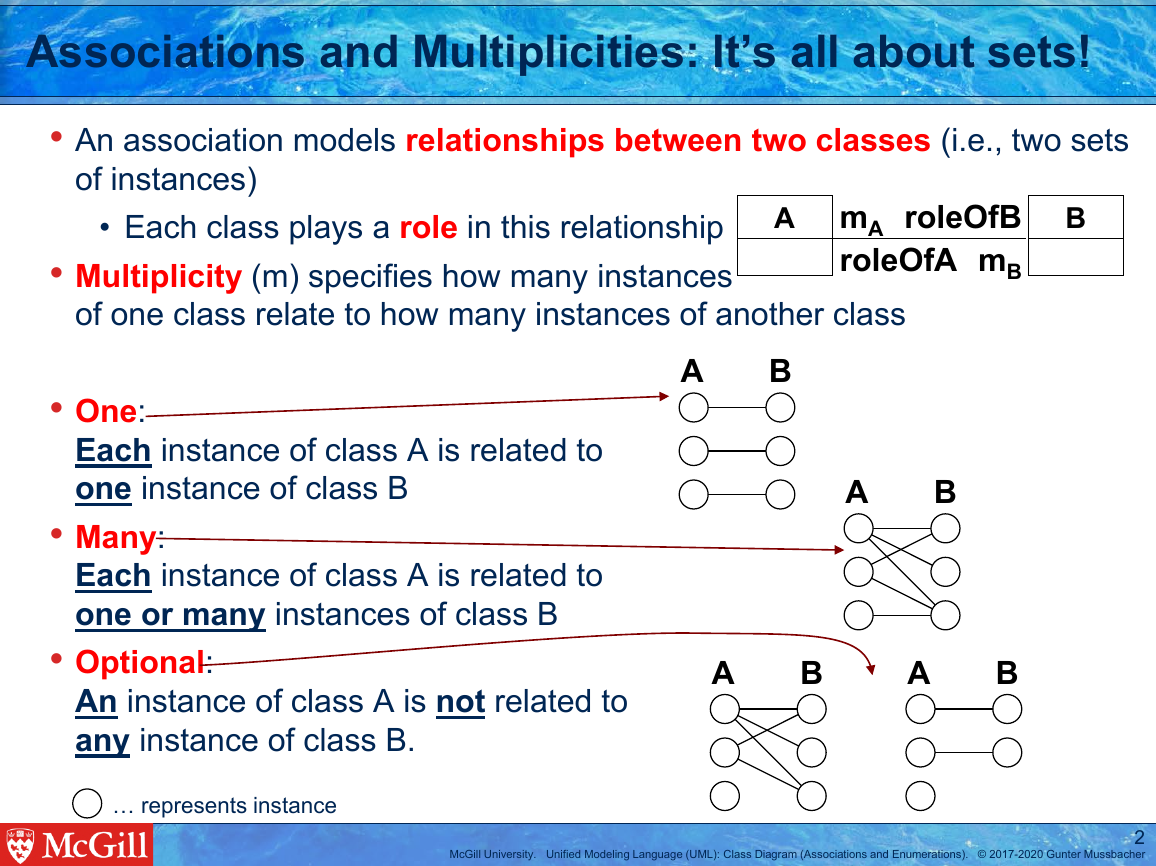
\includegraphics[width=0.6\textwidth]{images/role_name.png}
\end{tabular} \medskip


\subsection{Composition mistakes}

\subsubsection{Incomplete containment tree}

Student element: Classes.  \medskip

\noindent Level 1: Highlight solution  \medskip

\noindent Level 2: Text response: \medskip

\begin{tabular}{|p{0.9\linewidth}}
Please double-check the relationships of these classes.
\end{tabular} \medskip

\noindent Level 3: Parametrized response: \medskip

\begin{tabular}{|p{0.9\linewidth}}
\verb|${stud_cls*}| should be contained in the containment tree.[ Use composition for this.]
\end{tabular} \medskip

\noindent Level 4: Resource response with Example: \medskip

\begin{tabular}{|p{0.9\linewidth}}
Observe the following domain model. Every single class except the root class is directly or
indirectly contained in the root class, `PISystem`.

\\
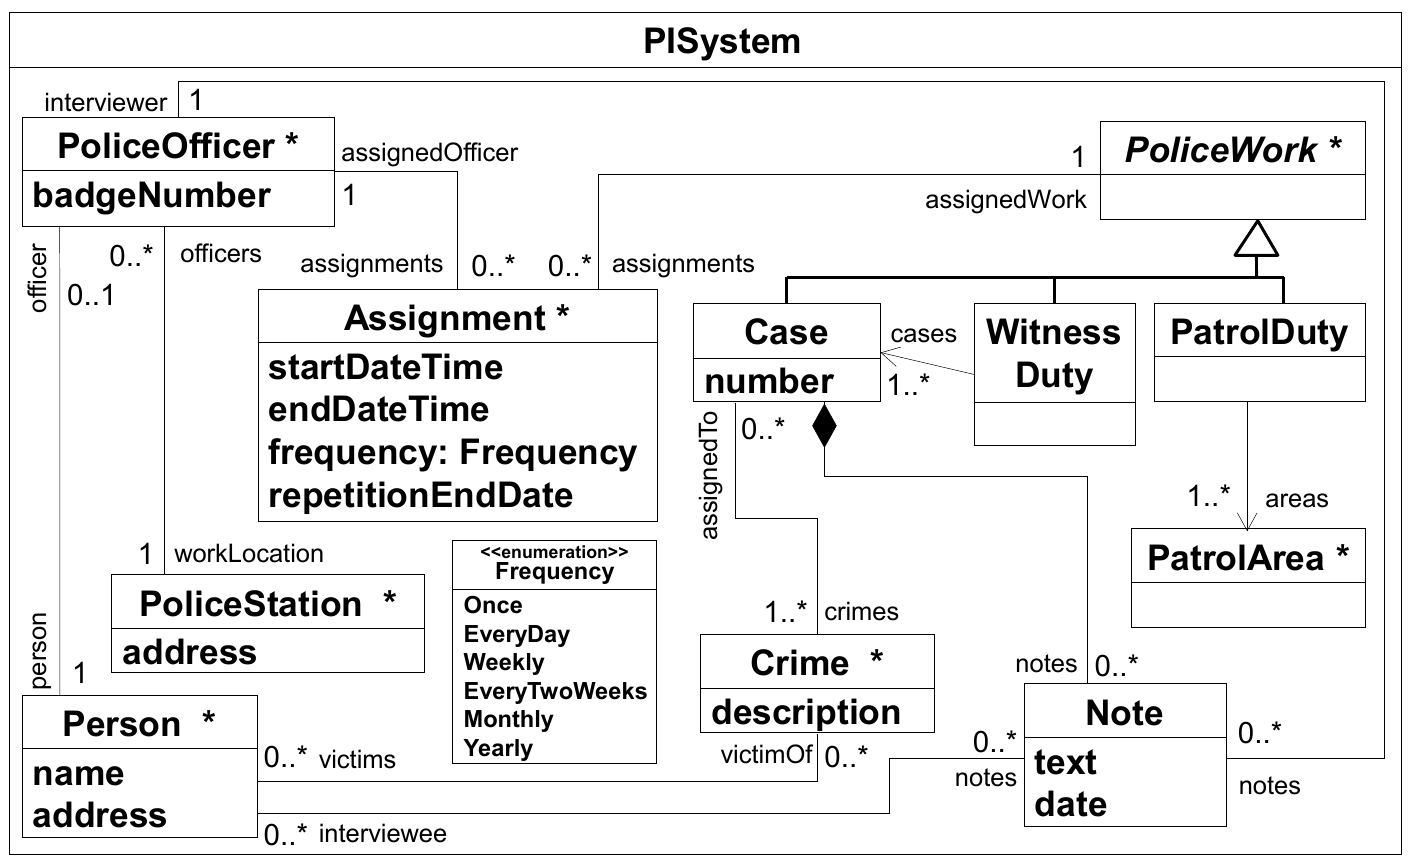
\includegraphics[width=0.6\textwidth]{images/PISystem.png}
\end{tabular} \medskip

\noindent Level 5: Resource response with List multiple-choice quiz: \medskip

\begin{tabular}{|p{0.9\linewidth}}

Which of the following compositions should be part of the containment tree for the following
model?

\\
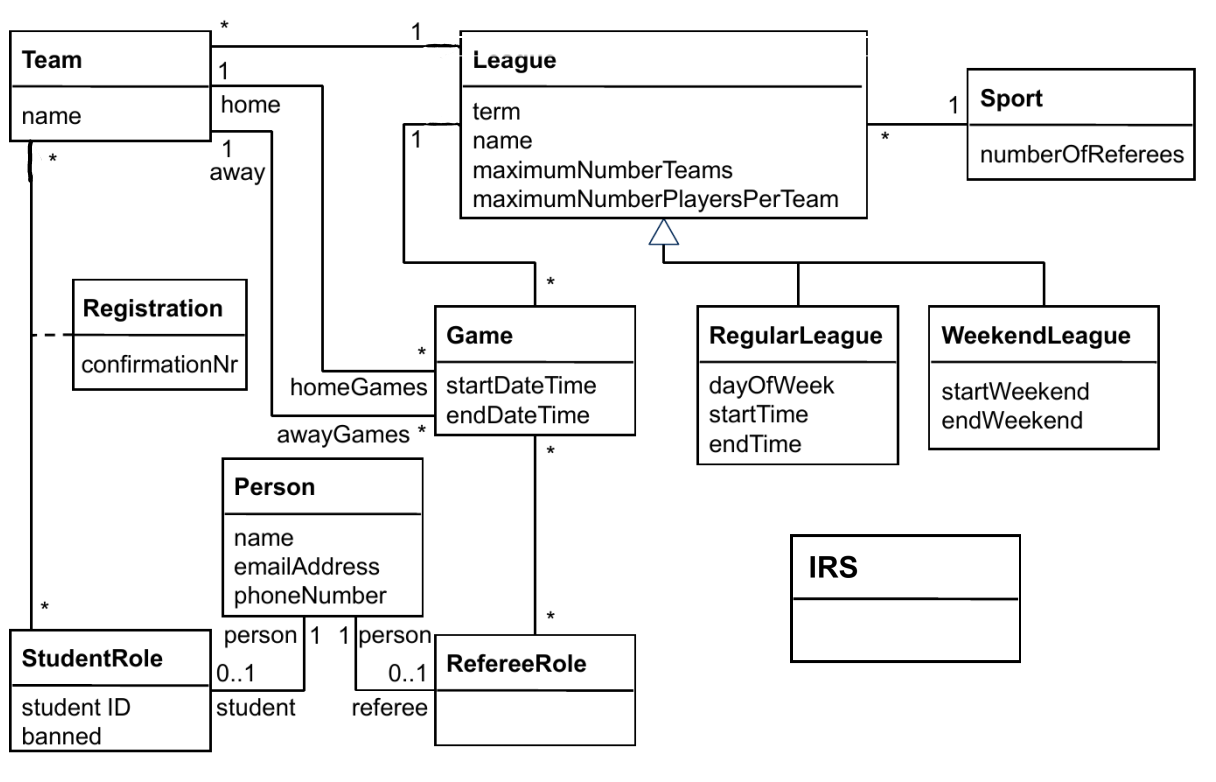
\includegraphics[width=0.6\textwidth]{images/IRS.png}

\begin{itemize}
    \item[$\boxtimes$] 1 IRS $<$@$>$- * StudentRole
    \item[$\boxtimes$] 1 IRS $<$@$>$- * Person
    \item[$\square$] 1 IRS $<$@$>$- * Game
    \item[$\boxtimes$] 1 IRS $<$@$>$- * League
    \item[$\square$] 1 IRS $<$@$>$- * RegularLeague
\end{itemize}

\end{tabular} \medskip

\noindent Level 6: Resource response with Reference: \medskip

\begin{tabular}{|p{0.9\linewidth}}
Please review the \textit{Composition vs. Aggregation vs. Association} section of 
the \textit{UML Class Diagram lecture slides} to 
better understand these relationships and where they are used.

\\
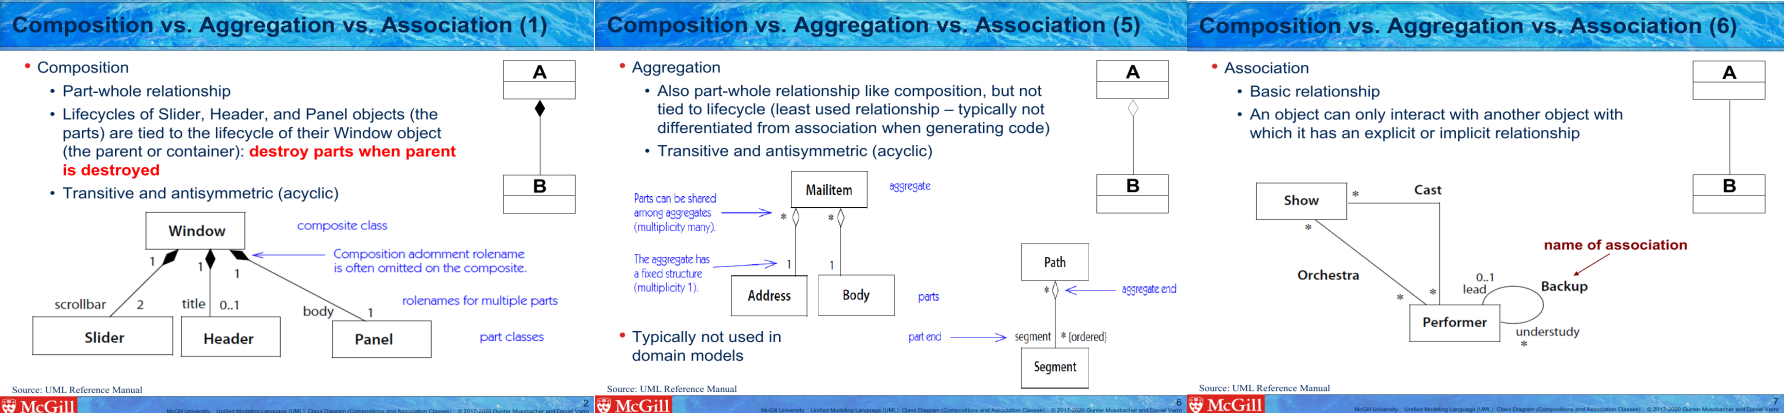
\includegraphics[width=0.9\textwidth]{images/composition_aggregation_association.png}
\end{tabular} \medskip


\subsection{Generalization mistakes}

\subsubsection{Missing generalization}

Instructor elements: Subclass, Superclass. \medskip

\noindent Level 1: Highlight sentence(s) in problem statement referring to the instructor element(s) \medskip

\noindent Level 2: Text response: \medskip

\begin{tabular}{|p{0.9\linewidth}}
What is the relationship between these classes?
\end{tabular} \medskip

\noindent Level 3: Parametrized response: \medskip

\begin{tabular}{|p{0.9\linewidth}}
A \verb|${inst_sub_cls}| is a \verb|${inst_super_cls}|. How should we model this?
\end{tabular} \medskip

\noindent Level 4: Resource response with Fill-in-the-blanks quiz: \medskip

\begin{tabular}{|p{0.9\linewidth}}

Place the following classes in an inheritance hierarchy: Vehicle, Wheel, LuxuryBus, Airplane, Car, Driver, LandVehicle, Bus. Only use a term once.

\begin{itemize}
    \item SportsCar isA \underline{Car}
    \item \underline{Wheel} isA VehiclePart
    \item Truck isA \underline{LandVehicle}
    \item AmphibiousVehicle isA \underline{Vehicle}
    \item \underline{LuxuryBus} isA BusVehicle
\end{itemize}

\end{tabular} \medskip

\noindent Level 5: Resource response with Reference: \medskip

\begin{tabular}{|p{0.9\linewidth}}
Please review the \textit{Generalization} part of the Class Diagram lecture.
\end{tabular} \medskip




\section{Design pattern mistakes}

\subsection{Abstraction-Occurrence pattern mistakes}

\subsubsection{Missing Abstraction-Occurrence pattern}

Instructor elements: Abstraction class, Occurrence class. \medskip

\noindent Level 1: Highlight sentence(s) in problem statement referring to the instructor element(s) \medskip

\noindent Level 2: Text response: \medskip

\begin{tabular}{|p{0.9\linewidth}}
Think carefully about how to model the relationship between these concepts.
\end{tabular} \medskip

\noindent Level 3: Parametrized response: \medskip

\begin{tabular}{|p{0.9\linewidth}}
The concepts of \verb|${inst_abs_cls}| and \verb|${inst_occ_cls}| and the relationship between them should be modeled with the Abstraction-Occurrence pattern.
\end{tabular} \medskip

\noindent Level 4: Resource response with Reference: \medskip

\begin{tabular}{|p{0.9\linewidth}}
The \textit{Abstraction-Occurrence Pattern} can be used to 
represent a set of related objects that share common information but also differ
from each other in an important way.

\\
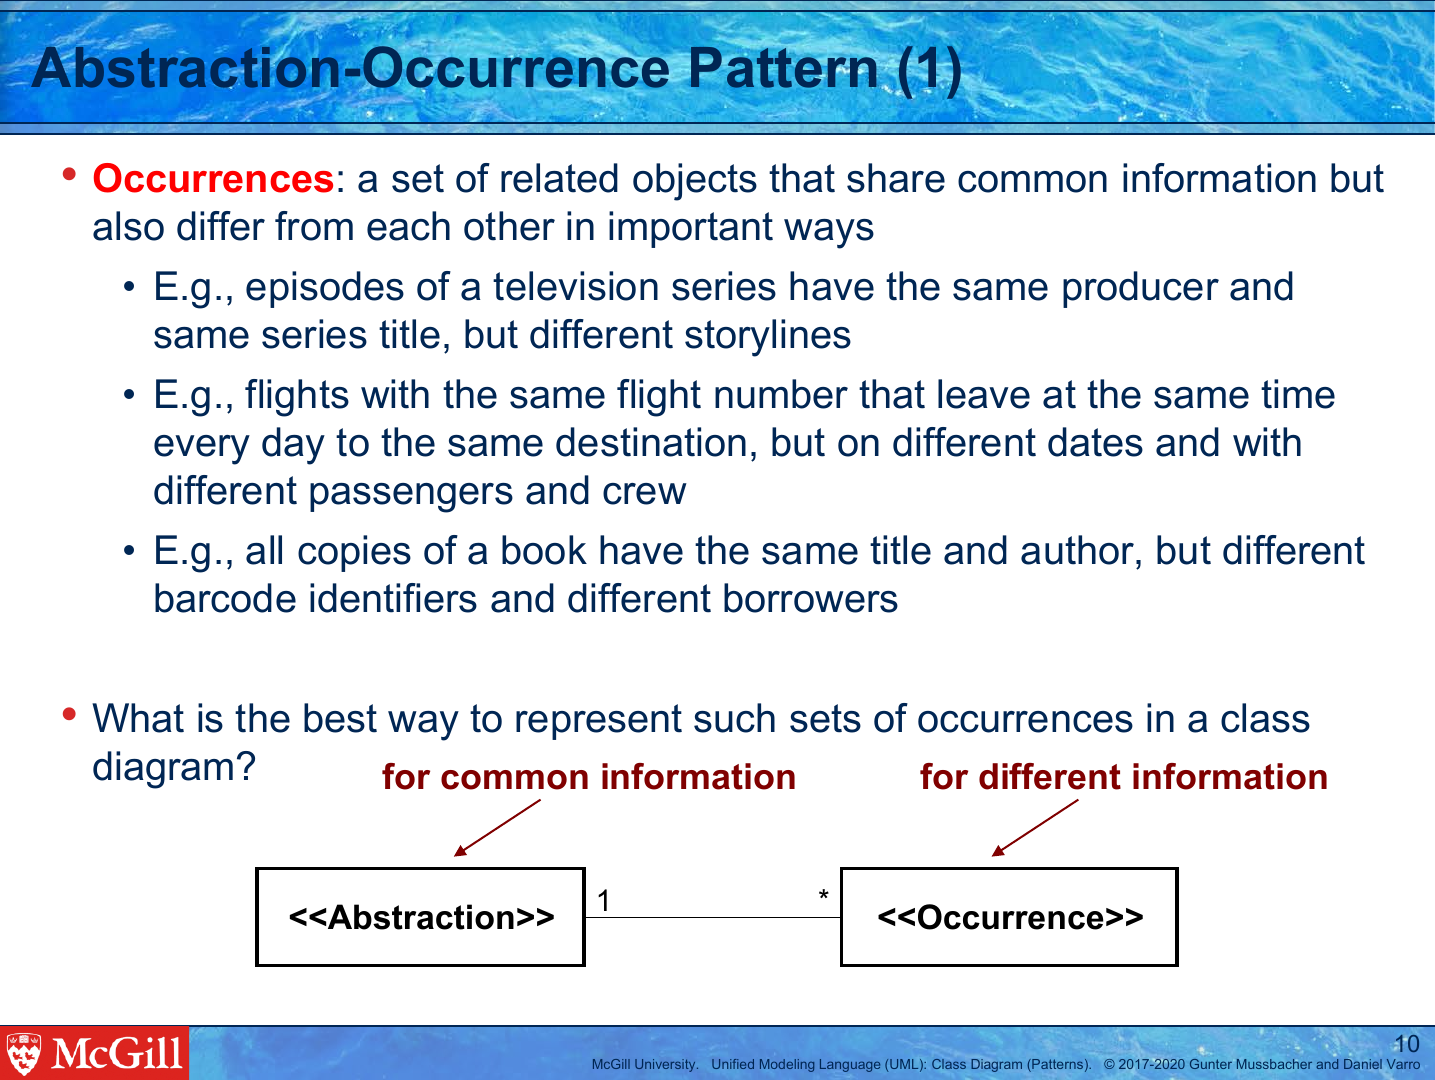
\includegraphics[width=0.6\textwidth]{images/abstraction_occurrence.png}
\end{tabular} \medskip



